%
% File acl2018.tex
%
%% Based on the style files for ACL-2017, with some changes, which were, in turn,
%% Based on the style files for ACL-2015, with some improvements
%%  taken from the NAACL-2016 style
%% Based on the style files for ACL-2014, which were, in turn,
%% based on ACL-2013, ACL-2012, ACL-2011, ACL-2010, ACL-IJCNLP-2009,
%% EACL-2009, IJCNLP-2008...
%% Based on the style files for EACL 2006 by 
%%e.agirre@ehu.es or Sergi.Balari@uab.es
%% and that of ACL 08 by Joakim Nivre and Noah Smith

\documentclass[11pt,a4paper]{article}
\usepackage[hyperref]{acl2018}
\usepackage{times}
\usepackage{latexsym}
\usepackage{graphicx}
\usepackage{booktabs}

\usepackage{url}

\aclfinalcopy % Uncomment this line for the final submission
%\def\aclpaperid{***} %  Enter the acl Paper ID here

%\setlength\titlebox{5cm}
% You can expand the titlebox if you need extra space
% to show all the authors. Please do not make the titlebox
% smaller than 5cm (the original size); we will check this
% in the camera-ready version and ask you to change it back.

\newcommand\BibTeX{B{\sc ib}\TeX}

\title{Graph Models of Named Entity Types\\for Interpretable Named Entity Disambiguation}

\author{Andrew Larimer \\
  {\tt andrewlarimer@berkeley.edu} \\\And
  Daniel Rasband \\
  {\tt danrasband@berkeley.edu} \\}
  
\date{12/07/18}

\begin{document}
\maketitle
\begin{abstract}
Like many neural networks, the decisions made by most Named Entity Recognition systems are difficult to interpret or adjust. We prototype a new Named Entity Recognition architecture that is very transparent and could be manually adjusted. Additionally, it is syntactically aware and focuses only on words with a direct dependency relationship to the entity in question, filtering out the noise of nearby words. Finally, our system builds a clear and cumulative 'mental model' of each named entity type, which may be extensible as a structure for persistent knowledge across long texts or for longterm knowledge-building.
\end{abstract}

\section{Introduction}
Named Entity Recognition systems have achieved impressive performance with state-of-the-art models resulting in ~90\% classification accuracy on popular benchmarks like the OntoNotes 5.0 corpus and the .

In order to achieve these results, however, the leading neural systems rely on matrices of numerical weights, often distributed across neural layers. This makes their rationale for arriving at a given classification uninterpretable by humans. While word embeddings, another mathematical construct of Natural Language Processing, can at least be explored in relation to one another by projecting them into 2D or 3D space, current NER systems don't provide us an easy way to compare the internal representations of different entity types.  In industries and applications that require decisions to be auditable, for example in the processing of loan applications that fall under the jurisdiction of the Fair Lending Act, the inability to peer into the workings of a model and clearly articulate why it is outputting one classification or another may not be acceptable.

We propose a novel graph-based architecture that allows for transparency in how a candidate entity is classified. While our prototype system currently achieves a much more modest accuracy of 40.23\% on the OntoNotes 5.0 corpus, we are confident that it can be further enhanced through the incorporation of additional input features and refinements. The basic validity of the approach is demonstrated by our model's significant performance over a baseline of always choosing the most common Named Entity Type ('ORG' in the OntoNotes 5.0 corpus) which would result in an accuracy of 18.03\% [ANDREW DOUBLE-CHECK THIS IN NOTEBOOK].

\begin{table}[t]
\begin{tabular}{@{}llll@{}}
\toprule
Model              & Corpus          & Type           & Accuracy        \\ \midrule
Lample et al. LSTM-CRF   &  CoNLL   & neural         & 90.94         \\
Lample et al. Stack-LSTM      &  CoNLL   & neural         & 90.33          \\
Chiu and Nichols   & OntoNotes          & neural         & 86.19          \\
Ratinov and Roth   & OntoNotes          & linear         & 83.45          \\ \midrule
\textbf{Our Model} & \textbf{OntoNotes} & \textbf{graph} & \textbf{40.32} \\ \midrule
Baseline           & OntoNotes          & baseline       & 18.32         
\end{tabular}
\label{tab:state_of_art}
\caption{Our model's accuracy currently lags behind other architectures, but surpasses a baseline of always choosing the most common entity type (ORG). The corpuses are more specifically CoNLL-2003 and OntoNotes 5.0.}
\end{table}

Our approach begins by training what we refer to as a Named Entity Template (NET) Graph. These graphs are intended to represent a 'mental model' or Platonic ideal of how this entity type interacts with the world (or at least how it is described as interacting with the world within text). Concretely, 

We achieve our results by first constructing a graph over a labeled training set that serves as a 'mental model' or 'Platonic ideal' of what a given Named Entity Type is. Concretely, Figure \ref{fig:person_graph} shows an example of a dramatically pruned version of our representation of the 'PERSON' entity type. The graphs are built to be grammatically aware, constructing a subgraph for each syntactic role the entity plays within the corpus. This allows for us to distinguish between what a given entity does in comparison to what is done to it.

In Figure \ref{fig:person_graph}, we see that when a 'PERSON' is the subject of a verb with an active tense, they might concede, dare, or sign something. When they are a direct object, someone might be urging them, bringing them somewhere, or handing them something. If used as a possession modifier, a person might have a widow, a son, or she might have words.

\begin{figure}[h]
  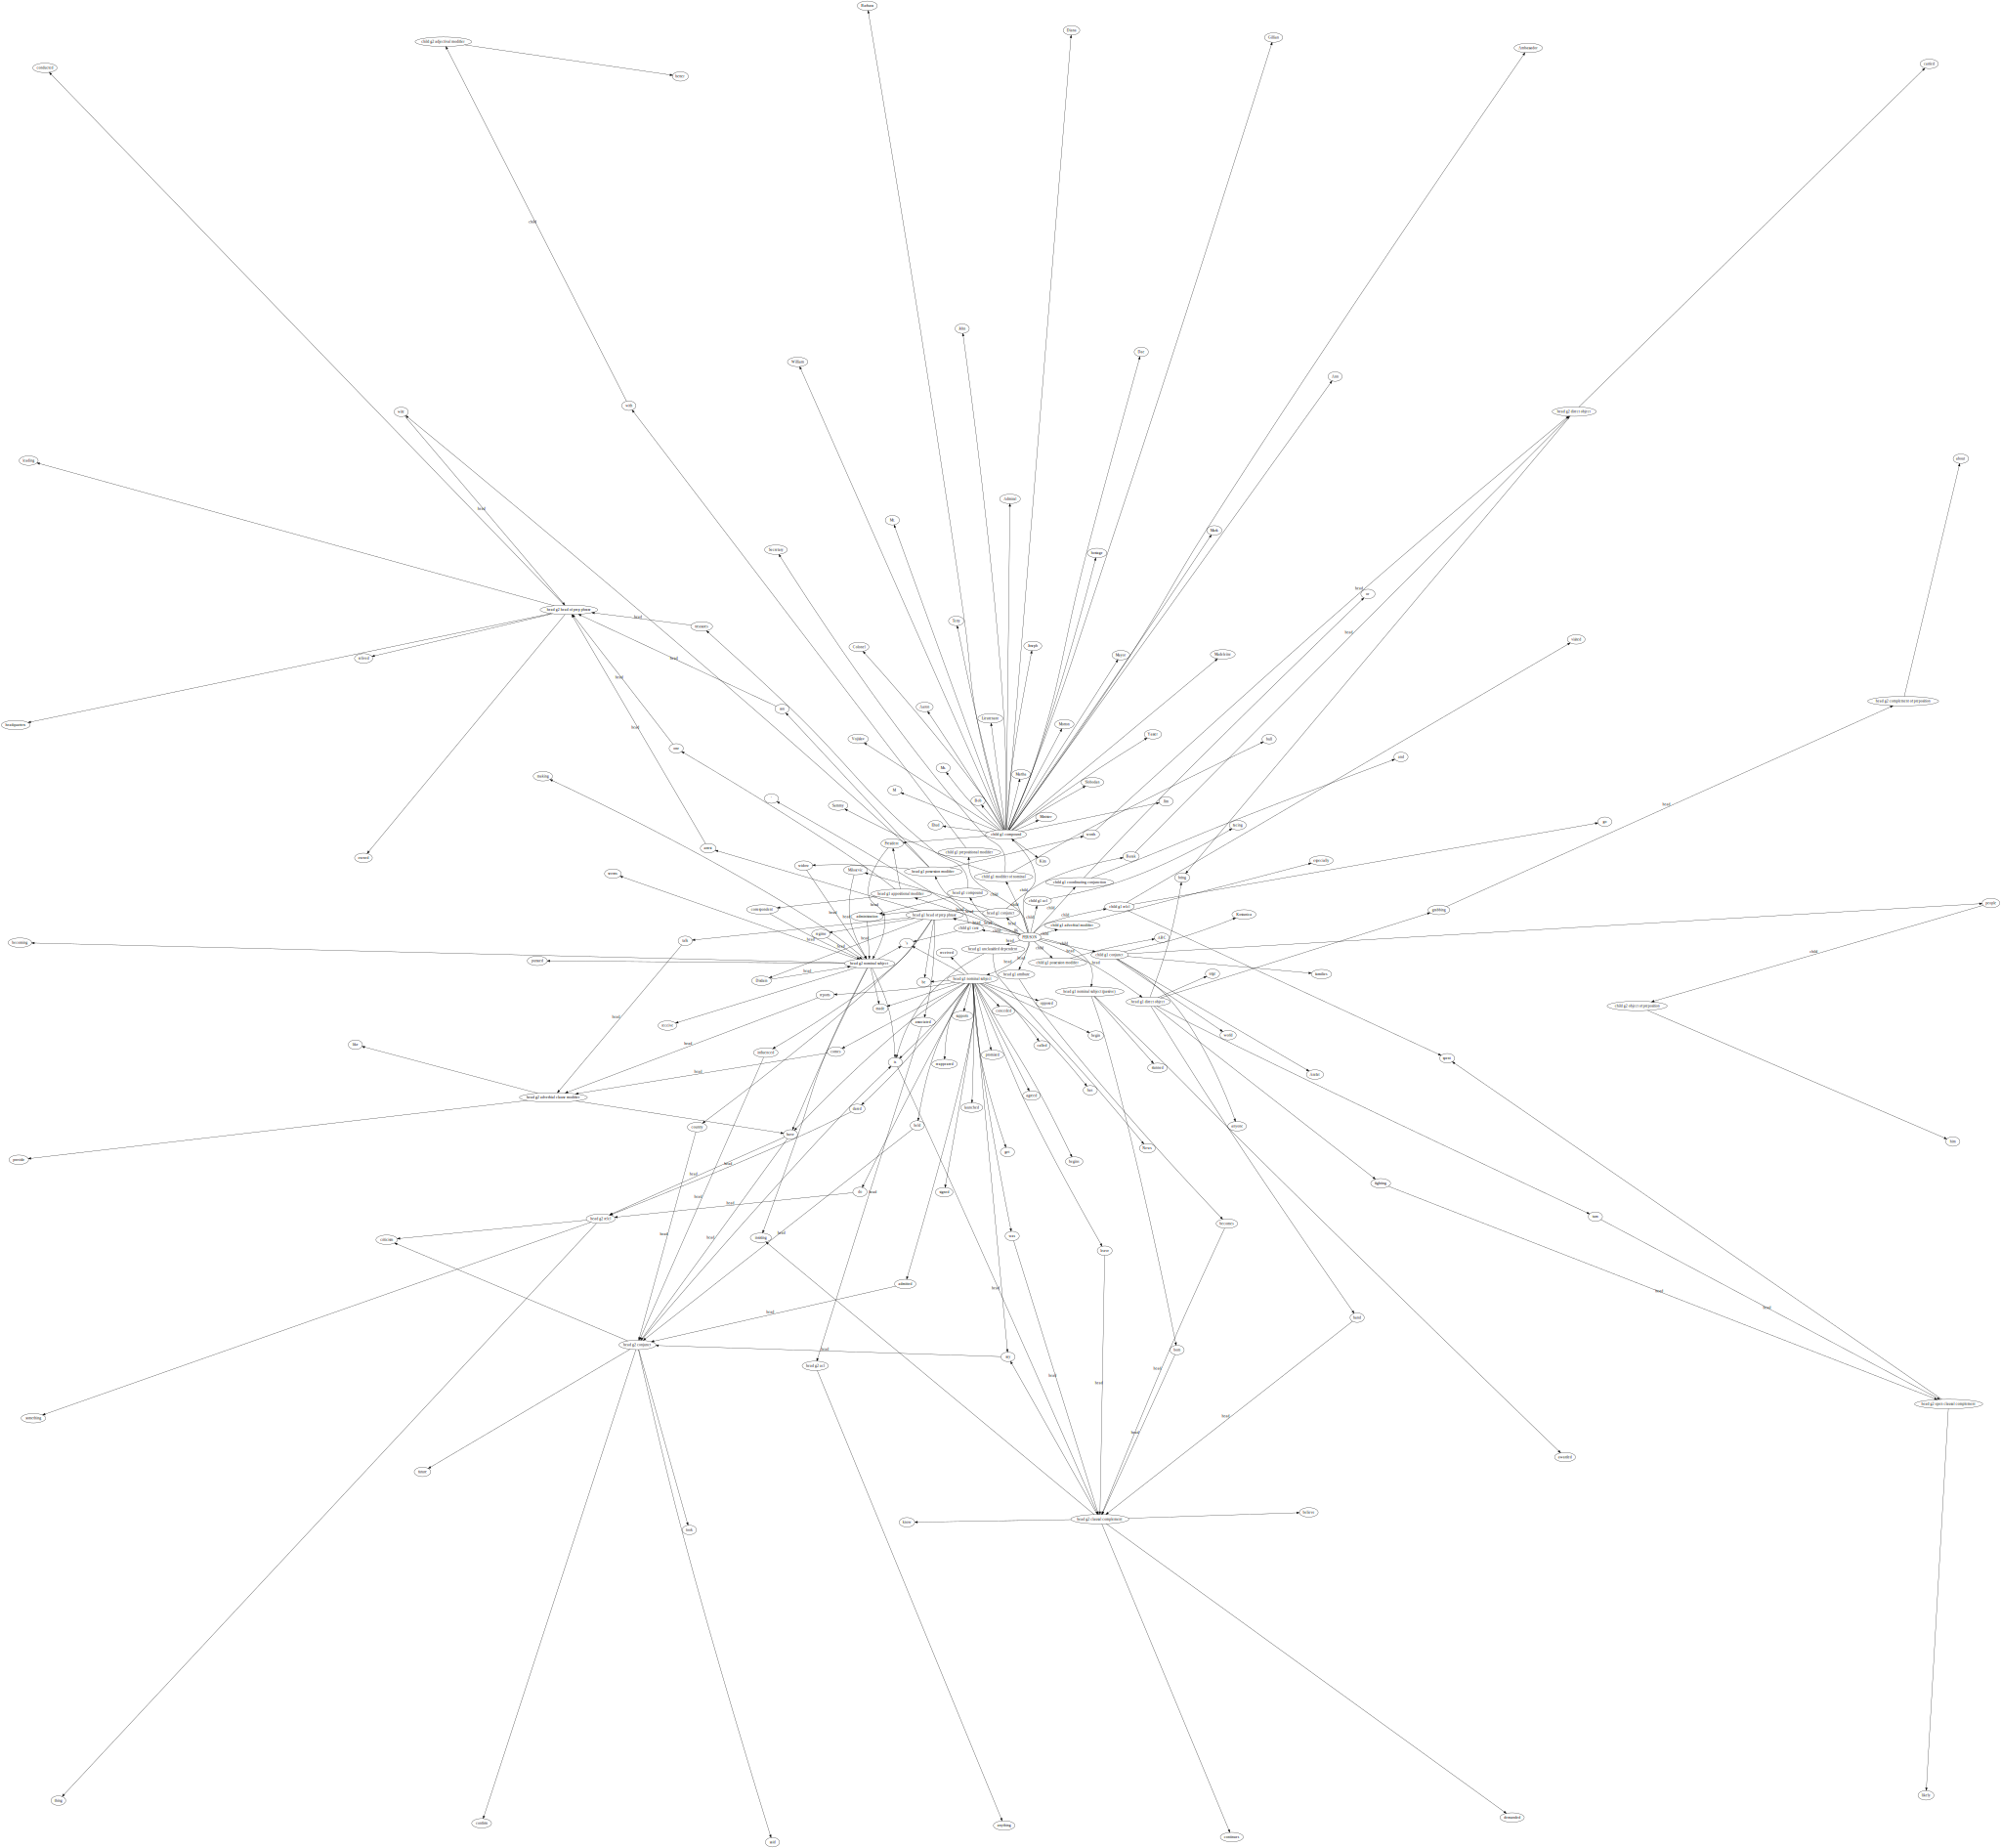
\includegraphics[width=\linewidth]{figures/G_PERSON.png}
  \caption{A simplified version of a Named Entity Type graph.}
  \label{fig:person_graph}
\end{figure}

The example in Figure \ref{fig:person_graph} shows a NET graph constructed from twelve occurences of entities labeled as 'PERSON' in the OntoNotes corpus. We use a depedency parser to parse each sentence in which a labeled entity occurs, and we create a leaf node from the word identified by the dependency parse as the head of our labeled entity. The dependency relationship between them, which is typically labeled on the arc in a visaulized dependency parse, becomes another node in between the root 'PERSON' node and its head in that occurence.

When conducting inference, we currently rely on an existing Named Entity Recognition system to supply candidates, and our system takes over to classify the candidate.

For each candidate entity, we construct a graph in a similar manner to how we construct the Named Entity Type graph. The primary difference is that while we have many labeled examples of a 'PERSON' in the OntoNotes corpus, when encountering a candidate entity, we only have its one concrete occurence. To supplement its graph, we use a coreference system to find other mentions in the text that represent the same entity, and add the relationships from each of those mentions to our graph.

We note here that while Figure \ref{fig:person_graph} shows only one generation of relationships in the direction of the dependency head, from a labeled entity to its direct head node according to a dependency parse, our NET graphs and candidate graphs actually traverse the dependency parse two generations up the tree (to the entity's head and that head's head) as well as two generations down the tree (to the entity's children, such as any adjectives modifying it, as well as the children of those children). This allows us to take in much more signal from the text that is still directly related to the entity we are considering.

Once a candidate graph has been construction, we compare it against each of our Named Entity Template graphs through a graph-similarity algorithm we developed. For our prediction we choose the label with the greatest similarity. In the case of a tie in maximum similarity scores, we choose the entity that occurs most frequently in the corpus from amidst the top scores.

We describe our process for building the graphs and computing their similarity further in Section \ref{methods}.

We think the virtue of this approach lies primarily in the transparency of the model. If desired, the system could easily be extended to include a reference point in the text for each node, for example, to point a reader to exactly which mentions in the corpus contributed to a model's interpretation.

Additionally, like any model, the more data it encounters the more robust each NET graph will become, and we believe that the interpretibility and generalizability of these graphs in describing the behavior and attributes of various entities might lead to them being utilized in other systems.

\section{Background and Related Work} \label{background}

While we ultimately decided to build a new architecture, we were informed and inspired by previous work directly related to NER as well as work from other subfields. In this section, we provide a brief survey of a few research papers and techniques and how they influenced our thinking.

\subsection{Transition-based NER}

\citet{LampleNeuralArchitecturesNamed2016} demonstrated interesting results in transition-based Named Entity Recognition. Using a similar model to a transition-based dependency parser, which processes text from left to right by considering one word at a time from a buffer of all the words in a sentence.

For each word it encounters, a traditional arc-standard transition-based system\cite{NivreIncrementalityDeterministicDependency2004} classifies the appropriate action to take from a small vocabulary of possible actions. One action in a transition-based system is a 'SHIFT' to move a word from the buffer onto a stack, which serves as both a storage area for words on which we are not yet ready to act, as well as a staging area for multi-word phrases. Another action in a typical dependency parsing transition-based system is 'REDUCE', which in arc-eager systems can come in a 'REDUCE-LEFT' and 'REDUCE-RIGHT' variety, and removes words from the buffer or stack depending on which directional varient is used, applying a dependency relation to the arc at the same time.

In this application, \citet{LampleNeuralArchitecturesNamed2016} used a similar system enhanced by Stack-LSTMs\cite{DyerTransitionBasedDependencyParsing2015} instead of simple stacks. An LSTM is a type of recurrent neural network that passes two outputs into another LSTM cell that shares its weights. One of these outputs is more directly responsive to the immediate input at each word as it moves over a text, while the other output called the 'cell state' is designed to carry signal until the chain of LSTM cells decides to alter it, thus enabling a longer 'memory' of the passage of text that has been fed through the network.The Stack-LSTMs used in this case are a hybrid of a stack data structure and a recurrent LSTM neural network designed such that each stack can maintain an embedded awareness of its full contents. And here, instead of applying dependency parse tags, they applied NER type labels upon a REDUCE action.

Transition-based approaches were intially designed to generate trees, and while it did not fall within the scope of this project, we think that if the utility of graph-based comparisons is further validated, using such a method to generate our candidate entity trees would be interesting to explore further.

\subsection{LSTMs and CRFs}

While we were particularly interested in the transition-based approach, we would be remiss in failing to discuss another architecture from the same paper\cite{LampleNeuralArchitecturesNamed2016} which had superior performance: a combination of bi-directional LSTMs and Conditional Random Fields.

In this model, the output of a pair of bi-directional LSTMs fed their output into a Conditional Random Field, which is a context-aware structure that is able to jointly model across the inputs from the sequence to capture the most likely NER tags across the sequence.

While their results of 90.46\% on the CoNLL-2003 corpus are impressive, they suffer from the lack of interpretability we discussed earlier.

\subsection{CNNs}
Fast and Accurate Entity Recognition with Iterated Dilated Convolutions. Strubell et al.

\subsection{Ontology-based NER}
As our specific approach might be described as existing somewhere between Named Entity Recognition and Knowledge Representation, we considered approaches from that subfield as well.

We found the work of \citet{SuciuInterleavingontologybasedreasoning2014} interesting in its Ontology-based approach for coming to understand characters and their actions in folktales. Concretely, 

\subsection{Separating identifying and validating candidate classifications}

While the field of Question Answering is distinct from NER, we were additionally inspired by the appraoch taken by \citet{HuReadVerifyMachine2018} in their approach to the Squad 2.0 Question Answering task. \cite{RajpurkarKnowWhatYou2018} Their approach focused on separating the tasks of finding the best candidate answer for a question, and then re-evaluating whether it in-fact answers the question. This inspired us to consider the steps of chunking named entities as distinct from classifying them, and we intend to further extend our model to be able to reject the sometimes over-eager candidates provided by named entity chunking systems.

\subsection{Comparing Graphs}
Algorithms for Graph Similarity and Subgraph Matching. Koutra et al.

\section{Methods} \label {methods}
We use the OntoNotes 5.0 corpus for its 143,709 sentences with labeled named entities.

\subsection{Creating our Named Entity Type Graphs} \label{construct_net}

Pre-treatment of the documents:
- Removing trace strings
- Converting digits

For each occurrence of a labeled named entity in that corpus, we do the following:

1. If this occurrence of a named entity consists of more than one word (ex. 'Nobel Peace Prize'), we assume the head of the phrase to be the last word of the named entity phrase.

2. We load the graph for the Named Entity Type represented by that occurrence (PERSON, ORGANIZATION, WORK OF ART, etc.).

3. We check to see if that Named Entity Type graph already has a child node corresponding to the dependency tag of the head of our named entity phrase. We call these nodes "syntactic function nodes."  In the 'Nobel Peace Prize' example, we see that 'Prize' is a 'direct object', so we find the 'direct object' child node of our 'WORK OF ART' entity type node. If there isn't already that child node, we create it. If it is already there, we increase a score count by one for the sake of generating weights later on.

We have implemented the dependency relationships as intermediary nodes rather than edges. First, it saves us time in inference by allowing us to use graph library methods to directly access the relationship nodes that represent how a given candidate entity we encounter is being used in a sentence. Additionally, it generates cleaner, more interpretable graphs, with natural clustering of the head words resulting from a particular syntactic usage of the entity type.

4. Under the appropriate "intermediary grammar node," we add a leaf node for our named entity's head in the dependency parse. In the "Nobel Peace Prize" example, the head of "Prize" when it was used as a direct object is "awarded," so we create a node for "awarded" as a child node of "direct object" and give it a score of one, unless it already exists, in which case we increase its score by one.

5. For the special case of arriving at a preposition, we take an extra arc to find the word that is that preposition's head, as we found more signal present in those head words than in the prepositions themselves.

6. After running through the corpus and building the graphs, we divide the score of each "syntactic function node" by the total occurrences of the named entity type to have weights between 0 and 1. We also normalize each leaf token's weight by dividing by its parent "syntactic function node"'s count, to also result in a weight from 0 to 1.

\subsection{Conducting Inference on a New Named Entity Candidate}

We consider each Named Entity as identified by an existing NER system (spaCy's built-in NER system) as a candidate, and do the following:

1. We construct a candidate graph in a similar manner to the one described above for generating the Named Entity Type (NET) graphs. We use a coreference system to include multiple references to the entity in order to have as robust a graph as possible to compare against our NET graphs.

2. We compare our candidate graph to each of the eighteen Named Entity Type graphs. For each leaf node in our candidate graph, we get its "syntactic function node", and so we focus our search on the child nodes of the Named Entity Type's corresponding syntactic function.

3. For each child node of that corresponding "syntactic function node," we calculate a score as follows: the similarity of the two words' embeddings (according to spaCy's Token.similarity() method, which is presumably a cosine similarity of the vectors but is not explicitly stated as such in their documentation) is multiplied by the weight of that leaf node in the Named Entity Type graph (which we calculated above based on its frequency of use within that grammatical context). By using the cosine similarity of the embeddings, we are more capable of performing inference on new candidate words that we don't find in any given Named Entity Type graph, but which may be similar. We are still considering how we will score a candidate word for which we don't have an embedding.

4. We sum the scores of each "syntactic function node"'s highest-scoring child node to arrive at the similarity score for that Named Entity Type Graph.

5. We compare the score of each NET graph, and choose the highest-scoring type which best matched our candidate graph as our prediction.

\section{Results and discussion}

We will develop our model on a dev set, and test our prediction accuracy against the labels in a held-out test set from the OntoNotes 5.0 corpus.

We will compare our performance against a baseline of the built-in spaCy NER module, which we will run on the same test set. Its performance is similar to other state of the art named entity recognition models, as seen in Figure \ref{tab:state_of_art}.



\subsection{Where our model worked well}

\begin{table}[h]
\begin{tabular}{@{}ll@{}}
\toprule
Entity Type & Our Accuracy \\ \midrule
ORG         & 40           \\
LOC         & 31           \\
GPE         & 20           \\
Log Prob    & 02          
\end{tabular}
\caption{Our accuracy on each Named Entity Type}
\end{table}

\subsection{Where our model failed}

\subsection{Possible enhancements}

Ideas for possible enhancements include:

\begin{itemize}

\item If it appears we are filtering out too much signal by being too selective, we are considering adding a hyperparameter that would not just take the immediate head and children of each entity in our NET graphs and inference candidates, but take one or two additional generations of head and child nodes, if they exist. This might allow us to take in more information while still filtering out noise that doesn't have a directly traceable dependency relation to the entity in question.

\item If inference is too slow due to the large size of the NET graphs, we have considered compressing the information in those graphs by clustering the leaf nodes using a Partitioning Around Medoids algorithm to find the 50 or so most representative leaf nodes and having those absorb the weights of the other members in their cluster, which we could then discard. We think this serve as a sort of regularization to allow the model to accept more synonyms rather than exact matches of candidates entity's heads to leaf nodes, while still maintaining the clarity of having real word leaf nodes.

\item Alternatively, if the model is too sensitive to whether a candidate entity's head matches exactly to a leaf node in our NET graphs, we could do clustering of the leaf node words via k-means, such that our clusters' centers would \textit{not} be actual words, but would exist somewhere in the embedding space near the words, and thus no word would likely be a 100\% match. To maintain interpretability, we could maintain a list of the closest leaf node to each cluster center.

\item We considered giving each syntactic function node a trainable weight, and then training those weights via a logistic regression type neural network to emphasize or deemphasize the importance of certain syntactic functions for classifying certain Named Entity Types, but we don't expect the candidate graphs to have enough different syntactic functions represented to make this worthwhile.

\item TF-IDF on the leaf nodes.

\item replace digits with DDDDD in the NET graphs

\item We are considering pruning stop words from the NET graphs, or using TF-IDF to dampen the weights of common words that might be found on several NET graphs (defining the graphs as the documents for purposes of the IDF).

\end{itemize}

\section{Conclusion}

We anticipate finishing our code for the above model in the next day or two, and then evaluating whether we have time to add possible enhancements.

We envision this system developing into a powerful classifier for longer literary works such as novels, particularly as we develop more fine grained named entity types.

In addition to being useful for interpretable Named Entity Disambiguation, the Named Entity Type graphs are interesting artifacts themselves, and we see additional possible uses for these techniques. One example use case might be in creating graphs that model the portrayal of different characters in a novel, for example, perhaps with a different graph for each chapter to help publishers and authors plot the development of characters over a longer work.

With additional refinement and the appropriate labeled dataset, we could classify a protagonist in a novel as a traditional hero or an anti-hero. We could identify occupations or literary tropes represented by supporting characters. And interesting tools for authors or publishers could be developed by tracking changes in a character's behavior from heroic to antiheroic from chapter to chapter.\cite{LampleNeuralArchitecturesNamed2016}

Furthermore, we see the potential of graph-based 'mental constructs' as having additional applications in the progression of machine learning. We believe transition-based parsing approaches could directly build on these graphs, and logical operations could be conducted on them to build out unstated but implied nodes that enhance our understanding of entities beyond what is explicitly stated. \cite{NivreIncrementalityDeterministicDependency2004}

% include your own bib file like this:
%\bibliographystyle{acl}
%\bibliography{acl2018}
\bibliography{acl2018}
\bibliographystyle{acl_natbib}

\end{document}
